In the current context, dominated by the advent of the Industry 4.0, production systems are characterized by a higher complexity of decision-making processes that are loosely distributed among the CPSs operating along the entire value network. 
It is time to envision interoperable simulation services capable to operate near the data sources to support first-time-right solutions to multi-disciplinary issues occurring in production, logistics and management processes.

This paper proposes four items that should lead the path of simulation technologies development to embrace and empower the digital transformation of industry. 
First, a virtual interoperable shop floor representation, relying on a shared modeling of core data that can be expanded to suit specific purposes, is required to sustain integration of different domains and provision of cloud-based simulation services. 
Especially SMEs, the least capable among industrial organizations to access the benefits of simulation, will profit from this democratizing approach that removes or reduces the adoption barriers while expanding the scope of simulation.
Interoperability of data models will pave the grounds for achieving situation awareness, the second item, that embodies the digital doppelganger (a.k.a. Digital Twin) concept to create live digital copies of the simulated environments and processes thus making it possible to oversee and control them on a factual basis.
The achievement of the first two items will allow simulation to take place in the loop of factory operations. This third item will dramatically change simulation's role from a predictive and testing technique that is used ex-ante to make decisions on possible designs, to a responsive and holistic system to support decision-making in real-time scenarios.
Finally, simulation models will need to be flexible and reconfigurable to leverage the smart nature of CPSs pursuing the plug-and-simulate condition, that is our fourth and last item. Plug-and-simulate makes adding new resources or modifying their behavior to be automatically or semi-automatically mirrored in the corresponding factory digital twin.
Supporting such ambitious objectives calls for a set of requirements that data models have to fulfill. To this end, our data model needs to be:
\begin{description}
\item[Expressive]- to enable the description of possibly any resource or flow involved in production, logistics and management processes of different industrial domains.
\item[Extensible]- to build, upon a core representation of the factory environment, a growing model ecosystem capable to maintain the digital information available all along the factory life-cycle.
\item[Interoperable]- to provide users with a personalized view and simulation tools that present the virtual environment from their perspective supporting the decision-making processes, activity planning and operation controlling.
\item[Scalable]- that is the ability to function efficiently when the context is changed in size or volume featuring multi-level access features and suitable aggregation patterns.
\item[Modular]- so that it provides representation building blocks that can be rearranged and reconfigured to follow the continuous evolution  of the real factory.
\end{description}


One of the most common features of manufacturing plant design is is to use standardized components (machine tools, robots, etc.) composed in a modular way. 
Through a good organization of modules, in fact, it is possible to speed up engineering as well as the simulation setups, maximizing the reuse of components. 
Similarly, simulation software solutions often provides libraries of models that can be aggregated and extended to assemble full plant layouts.
In this work we aspire to provide the same efficient re-use approach implementing classes to describe resources, called \textit{Archetypes} and \textit{Elements}. %which are instances of such elements and the components of the plant model. 
The Archetype-Element relationship is similar to the one that exists in Object Oriented Programming (OOP)~\cite{wolfgang1994design} between a Class and an Instance (Object) of that class.

Another important requirements is that the resulting data model shall support semantically meaningful collection of relations (referred to as \textit{Layers}). 
We deem particularly important to provide the modelers with a tool to gather links of the same type. 
The idea is to simplify the modeling process by dividing the overall model in several levels. 
By way of example, a first layer may contain the definition of the plant topology with its hierarchies of production resources; the other are graphs that can be used to express relations between resources. 
Logical, electrical, and pneumatic layers are just a few examples of layers.
Figure~\ref{fig:layers} illustrates graphically this multi-layer modeling approach. 

\begin{figure}
	\vspace*{-0.5cm}
	\centering
	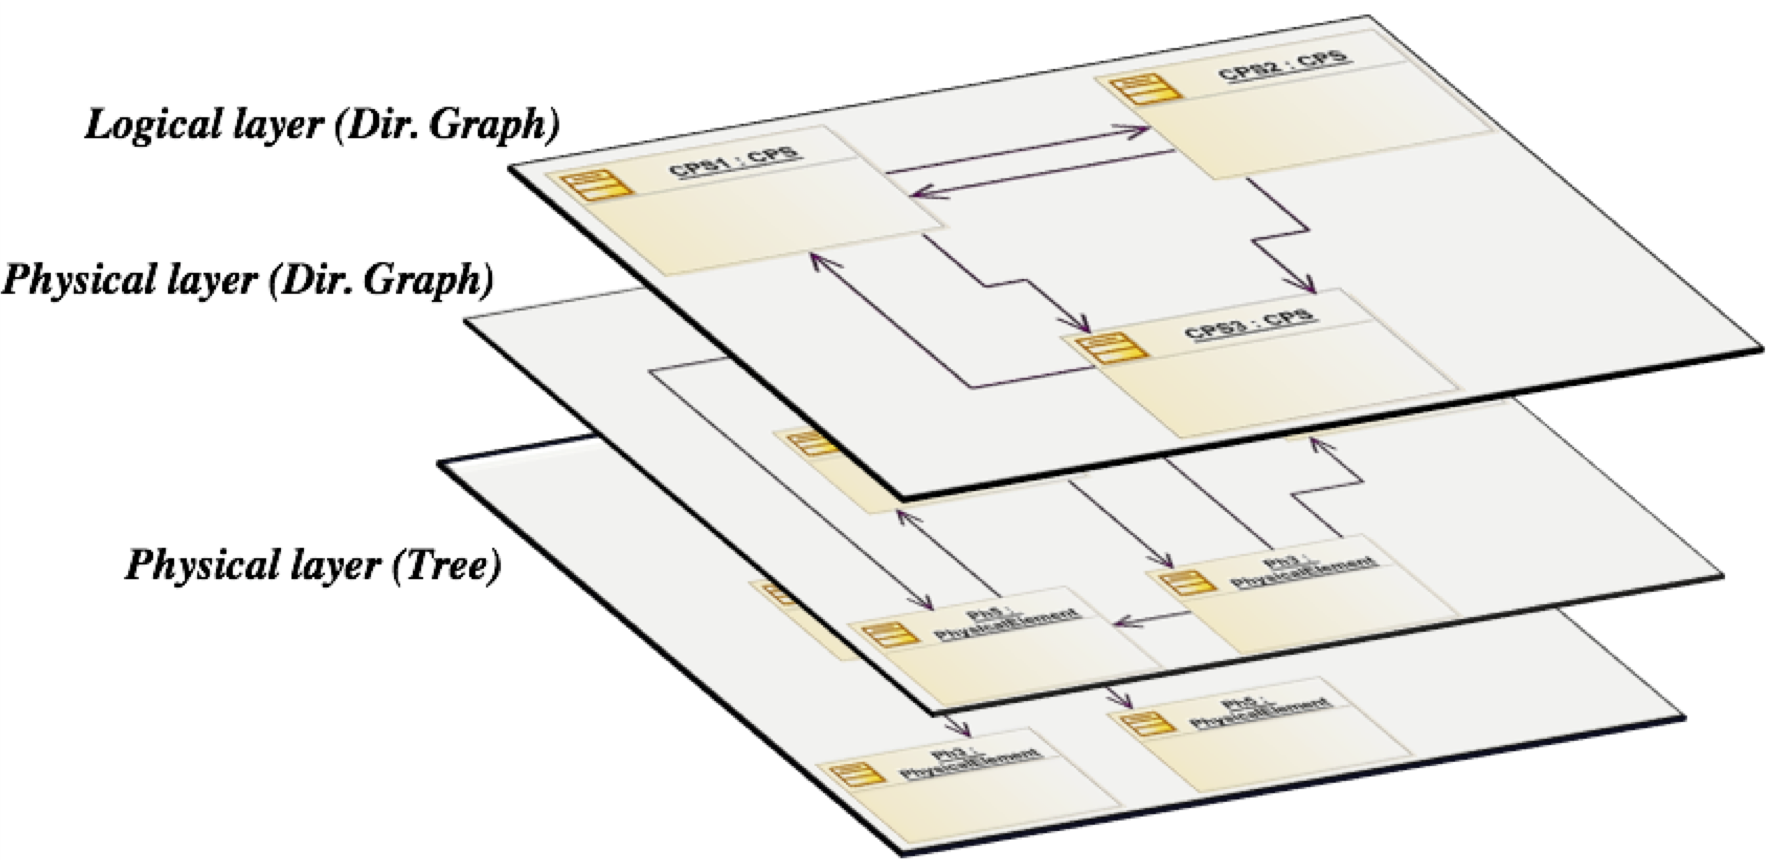
\includegraphics[width=\linewidth]{images/layers2}
	\caption{Modeling using superimposed layers}
	\label{fig:layers}
\end{figure}

This remainder of section documents the resulting data model for simulation, which is organized into 9 areas shortly described below:

\begin{description}
	\item[\textbf{Core Model}] - documents the core classes used for the definition of  entities and relations used in other sections.
	\item [\textbf{Archetype Model}] - introduces the concepts of Archetypes as the basis of the model reuse paradigm.
	\item[\textbf{Element Model}] - this model presents the concept of Element as instantiation of an Archetype according to the OOP.
	\item[\textbf{Connection Model}] - the connection model is devoted to the definition of the links between two model entities.
	\item[\textbf{Layer Model}] -  presents the concept of layer as a collection of items that can be further specified using attributes. 
	\item[\textbf{Attribute Model}] - specifies the concept of property to be used to annotate other elements of the model, namely Library, Archetype, Artifact, and Endpoint.
	\item[\textbf{Role Model}] - presents a set of classes that defined the concept of Role as semantic description to further specify the constituent elements of the model.
	\item[\textbf{Plant Model}] - introduces the Plant as an aggregation of layers representing among other aspects its physical and logical nature. 
	\item[\textbf{Project Model}] - documents all the classes that represent multi-plant simulation projects, and enable simulation tools to share plant models and results.
\end{description}
In this paper, nonetheless, due to the limited space available, only the main concepts and elements of the meta-model will be presented. 

